\documentclass[a4paper,12pt]{article}
\usepackage{graphicx}
\begin{document}

\vspace*{\fill}
\centerline{\huge \textbf{Documentation}} \hspace*{\fill}
\vspace*{\fill}
\\
\tableofcontents
\newpage

\section{Introduction}
This web application is a forum of questions and answers, akin to \emph{stackoverflow} and \emph{yahoo answers}. The web service will let a user find solutions to problems either by browsing the web site or asking a question oneself. Questions can be answered by other users and each answer can be rated. Highest rated solution offers are shown at the top. With enough questions and answers in the database, the service can provide a quick and convenient way to look up a solution for a problem of any kind. Tags can be added to the asked question to help browsing questions by category.\\
\indent Service will be hosted on university's users-server via Tomcat. Code will be written in Java via NetBeans IDE. App will use PostgreSQL database. User's browser will not require other scripts or plug-ins. Project has dependencies to \emph{Commons Fileupload} and \emph{Commons IO} packages.
\newpage

\section{General view of the application}
The following is an actor chart, followed with a description for each user and action.\\
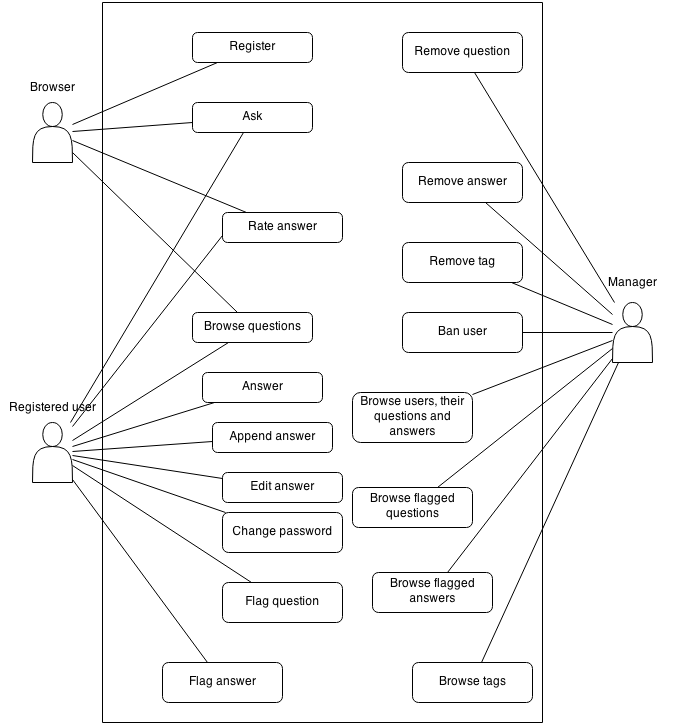
\includegraphics[scale=0.6]{ActorChart}

\noindent \textbf{Browser:} Unregistered user, that got access to the webapp simply by retrieving an url-link.\\
\textbf{Registered user:} User that has access to exclusive features by creating an account and logging into the app.\\
\textbf{Manager:} Webapp manager obligated to managing the forum, keeping it accessible to other users.\\

\noindent User actions:\\
\\
\textbf{Register:} Browser creates an account and promotes oneself into a registered user. User can then login to that account at any time if not banned.\\
\textbf{Ask:} User creates a question, awaiting a set of answers. Also sets tags for the question to improve the transparency of the question.\\
\textbf{Rate answer:} User marks answer as helpful and correct. Answer can also be rated down. Answer variant with most ratings is shown on top.\\
\textbf{Browse questions:} Lists questions. Tags can be specified to focus the search.\\
\textbf{Answer:} Adds an answer to a specified question.\\
\textbf{Append answer:} User edits one's answer by adding information into it.\\
\textbf{Change settings:} Registered user changes one's username, email, password and avatar.\\
\textbf{Flag question:} Notifies manager that specified question is inappropriate.\\
\textbf{Flag answer:} Notifies manager that specified answer is inappropriate.\\
\textbf{List own questions:} Lists questions that were asked by the user.\\
\textbf{List own answers:} Lists answers that were asked by the user.\\
\\
\textbf{Remove question:} Removes the specified question along with its answers.\\
\textbf{Remove answer:} Removes the specified answer.\\
\textbf{Remove tag:} Removes a tag from the database.\\
\textbf{Ban user:} Removes the user from the database. Questions and answers made by the user are spared, although their owner is marked as 'banned'.\\
\textbf{List users:} Lists users by join date with an option to ban them.\\
\textbf{List flagged questions:} Lists questions by their amount of flags. Helps finding inappropriate questions.\\
\textbf{List flagged answers:} Lists answers by their amount of flags. Helps finding inappropriate answers.\\
\textbf{List tags:} Lists tags. Whether they are inappropriate or not is apparent directly from the tag.\\
\newpage

\section{System's datacontents}
The following is a chart representing the required data contents of the system on a conceptual level:\\
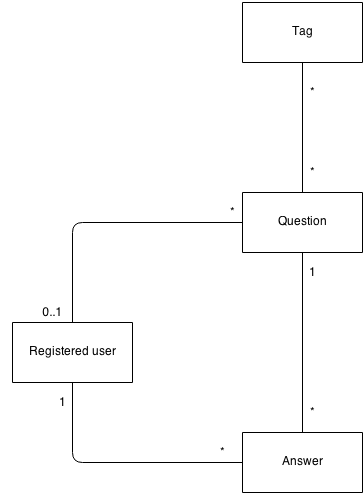
\includegraphics{ConceptChart}
\newpage
\noindent Four datablocks shown in the chart have following properties:\\
\\
\textbf{Datablock: Registered user}
\begin{center}
    \begin{tabular}{ | p{3cm} | p{4cm} | p{5cm} |}
    \hline
    Property & Value interval & Description \\ \hline
    Username & 16 characters & User's calling name in the forum. Can't be empty. \\ \hline
    E-mail & 64 characters & User's email to contact one. Can be omitted. \\ \hline
    Password & 128 bytes & User's hashed password to access the account. Can't be empty. \\
    \hline
    Salt & 16 bytes & Salt used to hash the password. Can't be empty. \\
    \hline
    Time user registered the account & Date and time &  \\
    \hline
    Moderator & Boolean & Notifies if user has moderator priviledges. False by default. \\ \hline
    Avatar & Picture file $\leq{256}$ kB, bytearray & User's picture to identify him by. Can be omitted. \\
    \hline
    \end{tabular}
\end{center}
\hspace*{\fill}\\
\textbf{Datablock: Question}
\begin{center}
    \begin{tabular}{ | p{4cm} | p{3cm} | p{5cm} |}
    \hline
    Property & Value interval & Description \\ \hline
    Question title & 96 characters & Question's essence displayed in search results. Can't be empty \\ \hline
    Question body & Any amount of text & Main part of the question. \\ \hline
    Asker is banned? & Boolean & In case if question has no owner, notifies whether question was asked anonymously or its owner was banned. \\ \hline
    Time when question was asked & Date and time &  \\
    \hline
    \end{tabular}
\end{center}
\newpage
\textbf{Datablock: Tag}
\begin{center}
    \begin{tabular}{ | p{4cm} | p{3cm} | p{5cm} |}
    \hline
    Property & Value interval & Description \\ \hline
    Tag title & 12 characters & Can't be empty \\ \hline
    Time when tagged & Date and time & Time when tag was first used. \\ \hline
    \end{tabular}
\end{center}
\hspace*{\fill}\\
\textbf{Datablock: Answer}
\begin{center}
    \begin{tabular}{ | p{4cm} | p{3cm} | p{5cm} |}
    \hline
    Property & Value interval & Description \\ \hline
    Answer body & Any amount of text &  \\ \hline
    Approved by asker & Boolean & True if poster of the question which this answer addresses has rated this answer. \\
    \hline
    Time when answer was posted & Date and time & This value is reset if answer is edited. \\
    \hline
    Time when answer was last edited & Date and time & \\
    \hline
    \end{tabular}
\end{center}
User can post multiple questions and answers. Each question and answer belongs to one user, although question may be posted anonymously, that way it won't belong to any user. Question may contain several answers. Each answer belongs to one question. Question may contain several tags and several question may be tagged with the same tag. User can flag several questions and answers. Questions and answers can be flagged by several users. User can rate several answers. Answer can be rated by several users as well as unregistered users.
\newpage

\section{Relation data base chart}
\hspace*{\fill}\\
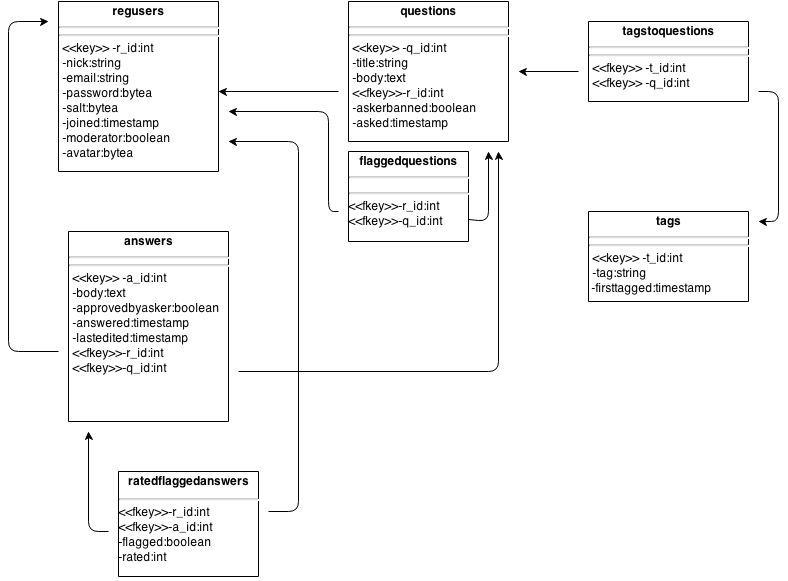
\includegraphics[scale=0.5]{RelationalDBChart}
\emph{Flaggedquestions} table restricts the user from flagging the same question multiple times. So does \emph{ratedflaggedanswers} table, however foreign key to \emph{regusers} can be set to null, allowing unregistered users to rate answers (but not flag). To restrict guests from rating same answer twice, rated answers are logged in the session. This can be exploited by manipulating sessions or by simply waiting for session's expiration time.\\
\emph{Ratedflaggedanswers} implements both rating and flagging an answer, which is toggled by \emph{flagged} field, which if set to true tells that answer was flagged, otherwise it's rated. Field \emph{rated} is set to 1, if answer was rated up, -1 otherwise.
\newpage

\section{System's architecture}
This app uses the traditional \emph{MVC-model}, meaning that the code is divided to three parts:\\
\emph{Models}, which access database data and stores it into objects.\\
\emph{Views}, which is client-side code mainly consisting of html-code.\\
\emph{Controllers}, which let correct users access correct app controls under correct premises.\\
\\
Models are stored in the Models package, which has four classes accessing four main database tables (registered user, question, answer, tag). Code for forming and closing connections with the database, properly preparing queries and managing returning results are placed at \emph{QAModel} class.\\
Views are stored in the \emph{web} directory, outside \emph{src} directory where most of the code is placed. Each webpage of the app is written in a .jsp file. Some parts of the html-code are stored in tag files, which are then referenced in .jsp files. These are placed at \emph{web/WEB-INF/tags}. Some .jsp files use customs tags located at \emph{CustomJSPTags} package.\\
Controllers are synonymous with Servlets in this app. These are placed in \emph{Servlets} package, controls exclusive to registered users are stored at \\
\emph{Servlets.RegisteredUser} and controls exclusive to moderators are stored at \emph{Servlets.Moderator}. Each concrete Servlet inherits QAServlet, which provides useful methods that are often used.\\
\\
\emph{Sessions} are used to store the user currently signed in, previous URL, guest's rated answers, error and info notifications. For example, if a user browses questions and only then decides to log in, after entering the information app redirects user to the question that was last browsed using the saved URL. When navigating to another page, app checks if user currently logged in still exists in the database. Notification strings are defined in \emph{utils} package. There also exists a class with static methods called \emph{Tools}, which has useful actions that can be used in many places of the code.
\newpage

\section{User interface}

The following is a map which represents all the sites that are accessible in the application, and what sites user can access next from the specified site:\\
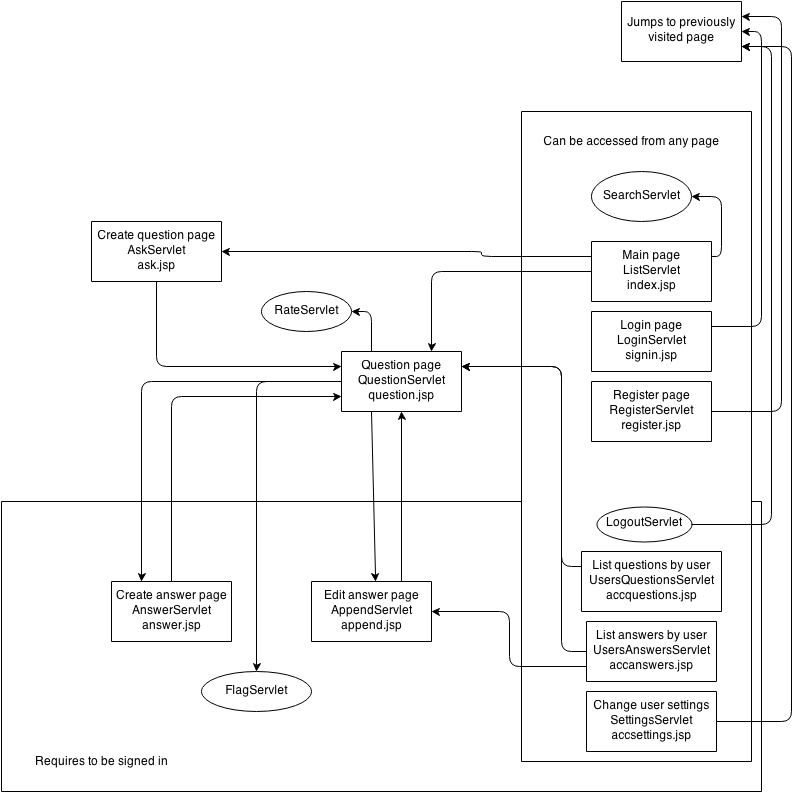
\includegraphics[scale=0.55]{sitemap2}\\
This is a design concept of the front page. Notice that it lists asked questions, offers user to ask a question, sign in or register.\\
\\
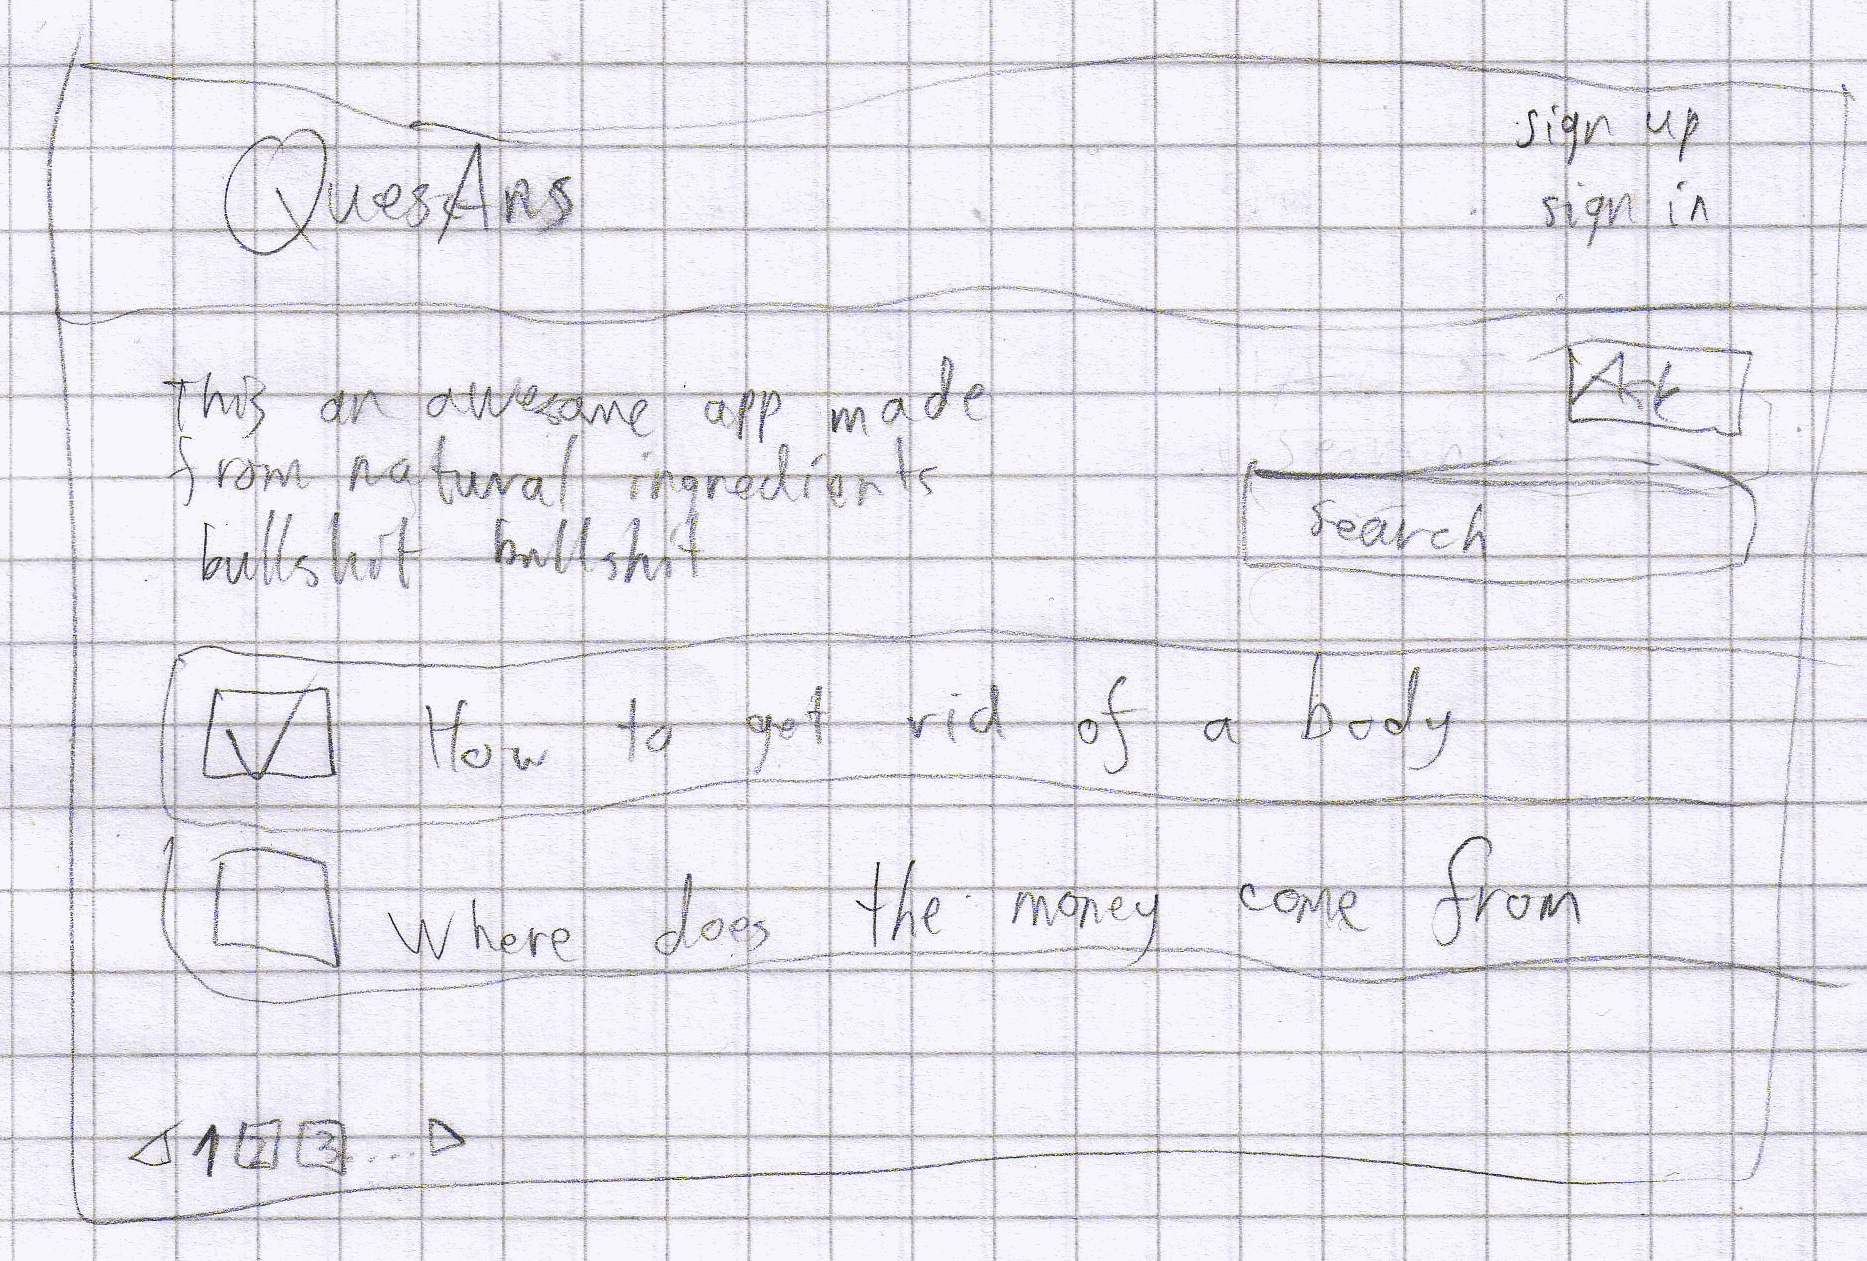
\includegraphics[scale=0.9]{FrontPage}
\newpage

\section{Installation}
To install the application, copy \emph{QuesAns.war} file to \emph{tomcat/webapps/} folder. Copying the file should be enough to make the tomcat unpack the file within the \emph{.war} file. \newline Next, configure \emph{context.xml} file at \emph{tomcat/webapps/QuesAns/META-INF/} to connect to the Postgres database. Use \emph{context.xml.dist} for reference. \newline
Now, as long as tomcat is running, web application should now be working. Run \emph{sql/create-tables.sql} in the database to set up correct datatables. Run \emph{sql/drop-tables.sql} to remove datatables.

\section{How to run and use the app}
Web application is accessed at the url: \emph{servername.com/QuesAns/}. At the moment of writing it is accessed at \emph{http://t-pasmpasm.users.cs.helsinki.fi/QuesAns/}. Press sign up at top-right corner to get started by registering a user. Notice that reading other questions, asking a question and rating answers doesn't require the user to be registered.

\section{Testing, ideas to improve the app}
Everything in the app was tested manually, therefore many bugs could have been ignored. As a new feature was implemented, it was tested immediately.\\
\\
All methods that access the database are static. This may cause concurrency problems, if several users are using the app at once. This was not tested. To make methods non-static would cause the app to establish a multitude of connections, blocking out access to the database. Reimplementation in that direction would require extensive redesign of connection code architecture.\\
\\
Many features were cut for time. Only user's own page can be accessed, while other users' pages can't be accessed in order to browse their questions and answers. This would've been useful for moderators. Search function in the main page only searches for questions by their tags. It would be more valuable to users if one can search questions by their title, search by answers and search users to access their pages.
\newpage

\section{Experiences while developing this app}
I learned a lot while developing this project as I have never done a webapp before. I learned a lot about restrictions involved with .jsp files, how it can and cannot access code. Few thing in coding stood out as particularly difficult, hardest things were to configure programs to work and to find time to develop the app while studying other courses.

\end{document}